
\section{Conclusions}
%Explain what conclusions you can draw from these set of experiments? The set of experiments and results reported here should justify some of the design choices described in the previous sections. (3-6 pages)
Figure  \ref{fig:exp-all-is} compares the Inception score for all tested network settings. Even though the Inception score of the basic DCGAN is not improved using the evaluated methods the overall quality of the generated images is clearly higher and the presence of mode collapse is significantly reduced or even non-existent for GAN's where spectral normalization, Wasserstein loss or both were added. In addition to these improvements both the D loss and G loss were much smoother during training. Having smoother losses allows for much better monitoring of the networks behavior during the training process leading to a much more intuitive hyper parameter tuning and debugging process. 
\begin{figure}[H]
\centering
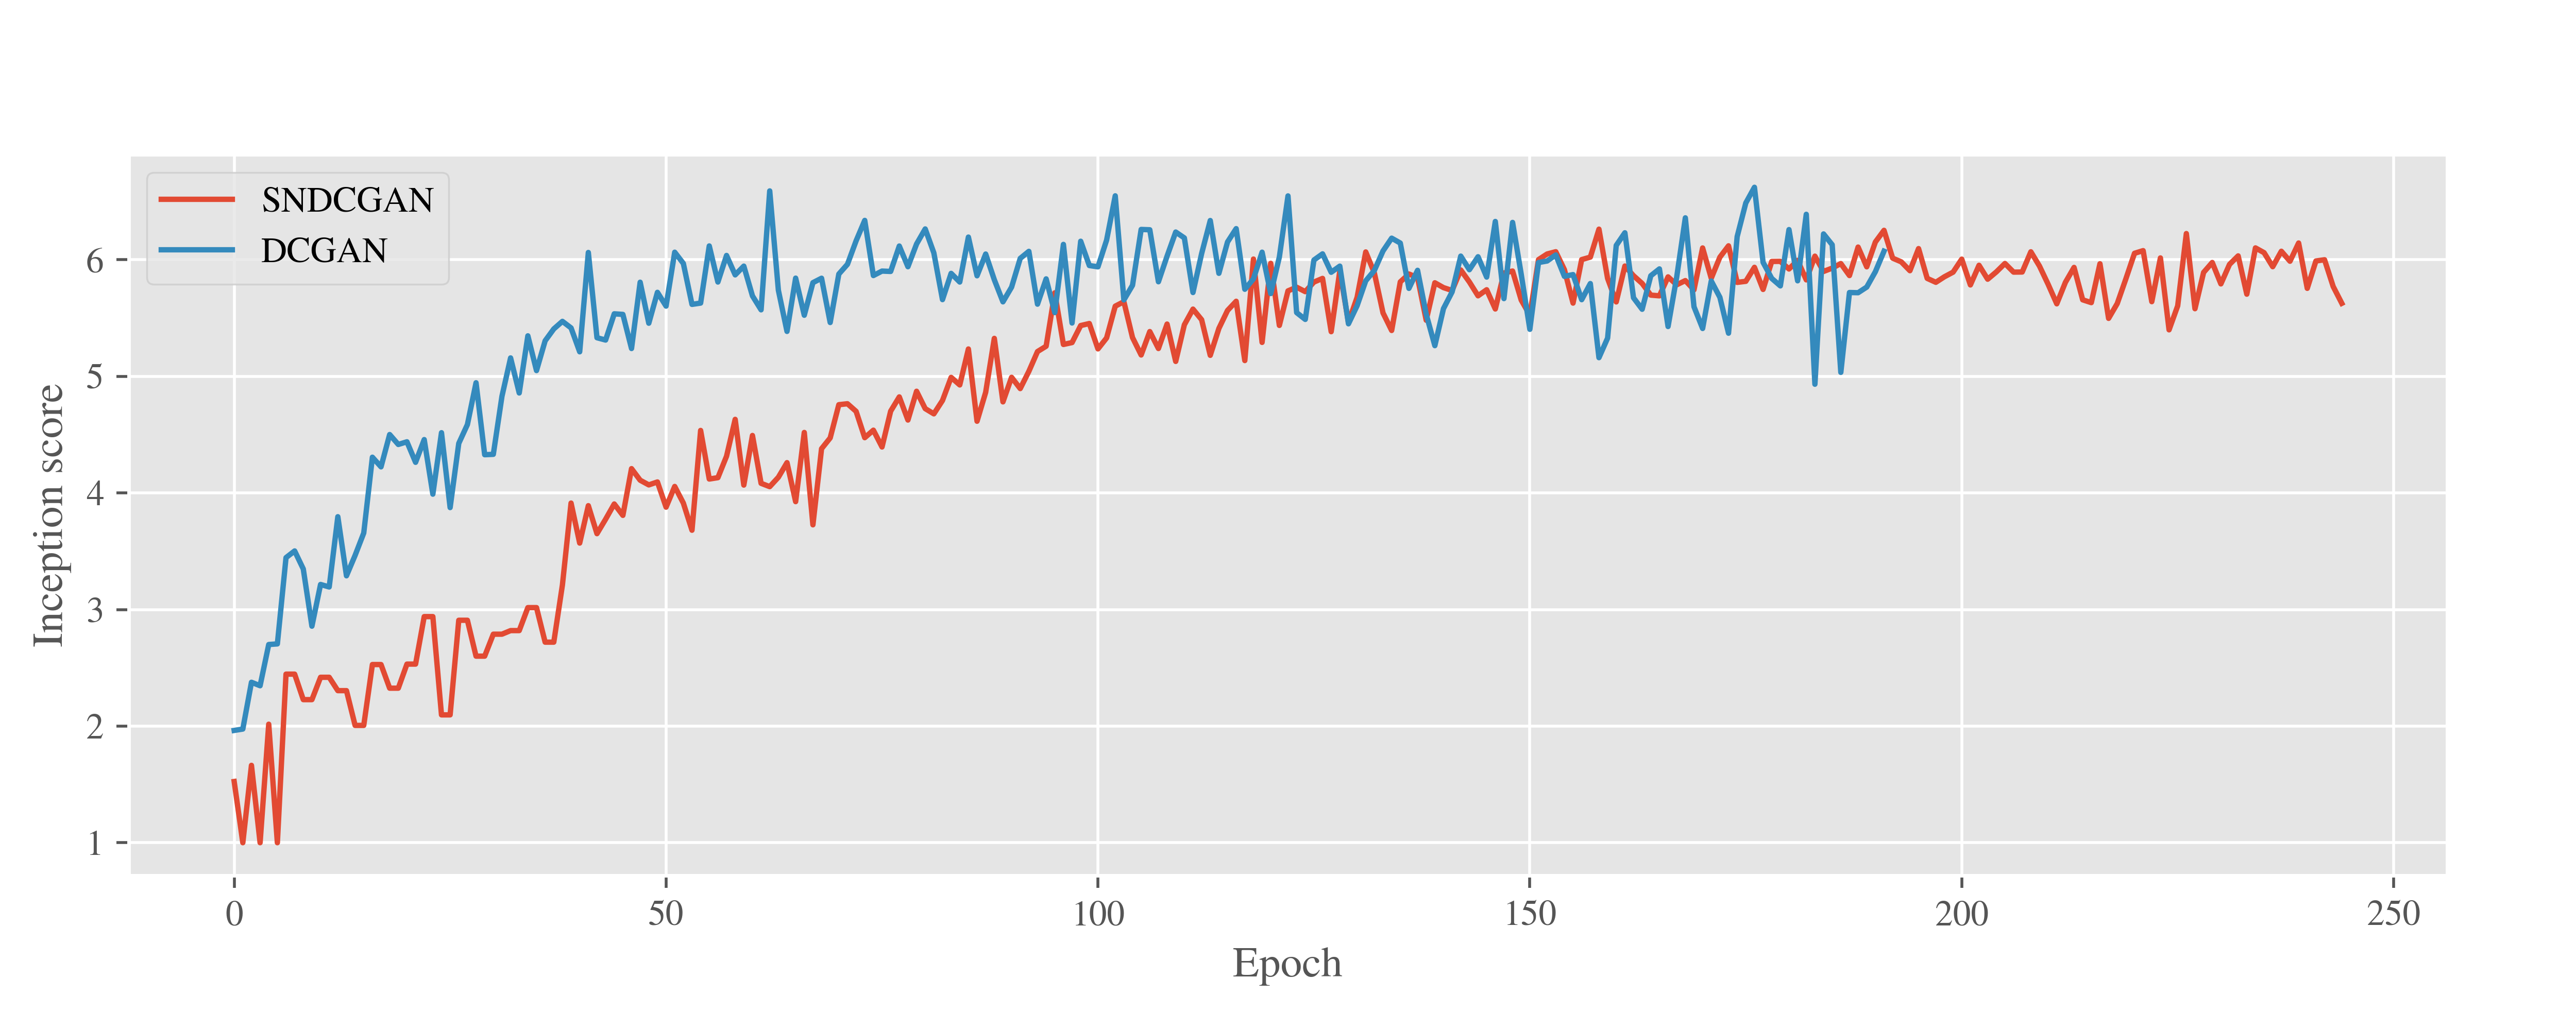
\includegraphics[width=\textwidth]{../code/results/figures/all_cifar10_is.png}
\caption{All evaluated models - Inception score, training on CIFAR10}
\label{fig:exp-all-is}
\end{figure}



%\todo{to justify the use of WGAN / the need for loss smoothness: Plotting these learning curves is not only useful for debugging and hyperparameter searches, but also correlate remarkably well with the observed sample quality. (taken from WGAN paper) }

\subsection{Future Work}
In the future, we would try and further explore the parameter space. The training of GANs is always a lengthy process with many influencing factors. With more time and resources, we would run parameter searches in a more systematic way and hopefully find better performing configurations. More specifically, we would start lower learning rates (ours might have been slightly too high; experiments show harsh loss evolutions) or different optimizers (WGAN literature advices to use RMSProp \cite{arjovsky2017wasserstein}).

Another contribution to our work would be to implement gradient penalty and run an experiment with Wasserstein loss as well. We expect that the performance of this configuration should fall in between that of our W-WC-DCGAN (weight clipping) and W-SN-DCGAN (spectral normalization).

Additionally, we would apply the same methodology to the LSGAN framework \cite{mao2017least} and see if spectral normalization can also help making training more stable. 
